\documentclass[article,10pt]{llncs}
\usepackage{makeidx}  % allows for indexgeneration

\usepackage[latin1]{inputenc}
%\usepackage[francais]{babel}
\usepackage{subfigure}
\usepackage{graphicx}
\usepackage{graphics}
\usepackage{dsfont}
\usepackage{natbib}
\usepackage{amsfonts,amsmath,amssymb}
\usepackage{enumerate}
\usepackage{stmaryrd}
\usepackage{color}
\usepackage{ulem}
\usepackage{float}
\floatstyle{ruled}
\usepackage{algpseudocode}
\usepackage{algorithmicx}
\usepackage{algorithm}
\usepackage{url}
\usepackage[table]{xcolor}

%\newfloat{Algorithm}{thp}{lop}
%\floatname{Algorithm}{Algorithm}
%\newtheorem{de}{Definition}[subsection] % les définitions et les théorémes sont
\newtheorem{theo}{Theorem}[section]    % numérotés par section
\newtheorem{lem}[theo]{Lemma}
%\newtheorem{cor}[theo]{Corrolary}
%\newtheorem{prop}[theo]{Proposition}

\newcommand{\soft}{\texttt{cghseg}}
\newcommand{\esoft}{\texttt{cghseg }}


\begin{document}

\title{High Dimension Segmentation using the \texttt{cghseg} package}
%
\titlerunning{High dimension with \texttt{cghseg}}  % abbreviated title (for running head)
%                                     also used for the TOC unless
%                                     \toctitle is used
%
\author{Guillem Rigaill$^1$, Vincent Miele$^2$ and Franck Picard$^2$}
%
\authorrunning{Rigaill et al.} % abbreviated author list (for running head)
%
%%%% list of authors for the TOC (use if author list has to be modified)
\tocauthor{G. Rigaill$^1$, V. Miele$^2$, F. Picard$^2$}
%
\institute{Laboratoire Statistique et G\'{e}nome, UMR CNRS 8071, USC INRA Universit\'{e} d'Evry, F-91037 Evry, France \\
\email{rigaill@evry.inra.fr},\\ 
\and
Laboratoire de Biom\'etrie et Biologie Evolutive, UMR CNRS 5558 Universit\'{e} Lyon 1, F-69622, Villeurbanne, France \\
\email{vincent.miele@univ-lyon1.fr},\\ 
\email{franck.picard@univ-lyon1.fr}
}

\maketitle   

\begin{abstract}
The method comes with a {\it next generation} \texttt{R} package, called \soft, which is fast enough to segment more than 1,000 profiles of length 100,000 in less than one afternoon.

\keywords{}
\end{abstract}

\section{Introduction}
\section{Linearization of Dynamic Programming for segmentation and segmentation/clustering} 

The purpose of segmentation is to partition a signal of $n$ observations $\{Y(t)\}$ into $K$ segments of homogeneous distributional parameter. In this section we deal with the univariate segmentation of one array CGH profile, the case of Joint multivariate segmentation being considered in Section 3. In the following a segment is an interval delimited by two change-points $\tau_k, \tau_{k+1}$ for instance,  with convention $\tau_0 = 1$ and $\tau_K = n+1$, and notation $r_k=\llbracket \tau_k, \tau_{k+1} -1\rrbracket$ stands for segment $k$. A segmentation in $K$ segments is denoted by $m^{(K)} = \{r_1, r_2 \ldots, r_K\}$.

A standard statistical model for segmentation is the detection of changes in the mean of a signal, such that $$\forall t \in r_k, \,\, Y(t)\sim \mathcal{N}(\mu_k,\sigma^2).$$ In the special case of array CGH, an additional step is the ``calling step'' that is performed by introducing additional (hidden) label variables $\{C(r_k)\}_k$ to cluster each segment into categories such as \texttt{deleted}, \texttt{normal}, \texttt{amplified} (not limited to 3 states). Then the segmentation/clustering model becomes  $$\forall t \in r_k, \,\, Y(t)|\{C(r_k)=p\} \sim \mathcal{N}(\mu_p,\sigma^2),$$ with $p=1,...,P$, $P$ being fixed.

Once the statistical model has been defined, the main algorithmic challenge lies in the exact detertination of the boundaries of segments $\{\tau_k\}$ (and not in the estimation of mean parameters $\mu_k$s or $\mu_p$s depending on the model). A well known solution to this problem is to use Dynamic Programming for a given number of segments $K$. Note that in this work, we do not deal with the statistical issue of model selection to estimate $K$ and $P$. We use appropriate model selection criteria that have already been published and discussed elsewhere.

To perform Dynamic Programming, we need to define the ``unit'' cost of a generic segment $r = \llbracket t_1, t_2 \rrbracket$, whose cost function is given by minus the local log-likelihood calculated on $r$:
$$ C_{t_1, t_2}^{(1)} =C_{(r)}^{(1)} = 
\begin{cases}
\sum_{t \in r} (y(t) - \mu_r)^2/2 \sigma^2 \text{, for segmentation in the mean}  \\
-\log\left(\sum_p \pi_p \exp \left\{ - \sum_{t \in r} (y(t) - \mu_p)^2 / 2 \sigma^2 \right\}\right) \text{, for seg/clust}.
\end{cases}
$$ 
A main difference between the two models lies in the estimation of the mean parameters. In the case of segmentation in the mean, parameters $\{\mu_k\}_k$ can be estimated directly by the empirical means of segments while computing the position of the breaks. In the case of segmentation/clustering, parameters $\{\mu_p\}_p$ are common across segments. Consequently, they are fixed while computing breakpoint coordinates, and they are estimated iteratively by using an EM-algorithm, leading to a DP-EM algorithm \cite{picard_2007}. 

In the case of segmentation/clustering, we propose to simplify the cost function by using a \textit{classification loss}, an approximation denoted by $\widetilde{C}_{(r)}^{(1)}$ which consists in focusing on the dominant term within the sum over $P$ exponentials:
\begin{equation}
\label{Eq:approx}
\widetilde{C}_{(r)}^{(1)}= \min_p \left\{ \sum_{t \in r}\frac{(y(t) - \mu_p)^2} {2\sigma^2 } + \log(\pi_p)\right\}.
\end{equation}

Since the purpose is to find the global minimum of the total cost function into $K$ segments, we also introduce the set of all segmentations of a given segment $r$ into $K$ segments such that $\mathcal{M}^{(K)}_{(r)} = \mathcal{M}^{(K)}_{t_1, t_2}$. Then the optimal cost of a segmentation of $r$ into $K$ segments and its associated optimal segmentation are defined as:
$$
C_{t_1, t_2}^{(K)} = C_{(r)}^{(K)} = \min_{m \in \mathcal{M}^{(K)}_{(r)}} \left\{ \sum_{r \in m} C^{(1)}_{(r)} \right\}, 
\text{ and }
\widehat{m}_{t_1, t_2}^{(K)} = \widehat{m}_{(r)}^{(K)} = \underset{m \in \mathcal{M}^{(K)}_{(r)}}{\operatorname{argmin}} \left\{ \sum_{r \in m} C^{(1)}_{(r)} \right\}.
$$
Similarly, we use notations 
$$
\widetilde{C}_{(r)}^{(K)} =\min_{m \in \mathcal{M}^{(K)}_{(r)}} \left\{ \sum_{r \in m} \widetilde{C}^{(1)}_{(r)} \right\}, \text{ and }
\widetilde{m}_{(r)}^{(K)} = \underset{m \in \mathcal{M}^{(K)}_{(r)}}{\operatorname{argmin}} \left\{ \sum_{r \in m} \widetilde{C}^{(1)}_{(r)} \right\}
$$
when approximation (\ref{Eq:approx}) is used.\\

When the cost or loss of a segmentation is segment additive (which is the case in both models), a $\mathcal{O}(Kn^2)$ Dynamic Programming algorithm can be built to recover the best exact segmentation (into $1$ to $K$ segments).

\subsection{Original Dynamic Programming algorithm for segmentation}

A basic statement is that the cost of a given segmentation is the sum of the cost of its segments. Thus the Bellman optimality principal holds and we have: $ C_{1, t}^{(k+1)} = \min_{\tau \leq t} \{ C_{1, \tau -1}^{(k)}  + C_{\tau, t}^{(1)} \} .$
%More generally for any $k_1 (>0)$ and $k_2 (> 0)$   we have %$$ C_{1, t}^{(k_1 + k_2)} = min_{\tau \leq t} \{ C_{1, \tau -1}^{(k_1)}  + C_{\tau, t}^{(k_2)} \} $$
Using this update rule  a Dynamic Programming algorithm can be built to recover all $ C_{1, t}^{(k+1)}$ for all $t \leq n$ and $k \leq K$.
This can be done using Algorithm \ref{algo:DPA2} for instance. 
For simplicity we did not include the initialization of all $C^{(1)}_{1,t}$ for $t \leq n$ and of all $C^{(k)}_{1,t}$ for $k \leq K$ and $t < k$.
All $C^{(k)}_{1,t}$ are initialized as $+\infty$ and $C^{(1)}_{1,t}$ are initialized using their definition.
This algorithm assumes that all $C_{t_1, t_2}^{(1)}$ have been pre-computed and stored (in 
a $n$ by $n$ matrix) or that they can be efficiently computed on the fly, which is the case for every models we consider here. At step $k, t$ of Algorithm \ref{algo:DPA2}  $\mathcal{O}(t)$ basic operations are performed. If we sum these for all $k < K$ and $t < n$  we see that the algorithm has a $\mathcal{O}(Kn^2)$ time complexity. This $n^2$ factor is the main reason why Dynamic Programming can be prohibitive to use on large signals (like SNP arrays for instance).

\begin{algorithm}
  \caption{Standard Dynamic Programming algorithm}\label{algo:DPA2}
  \begin{algorithmic}
    \State \textbf{Input}: $Y(t)$ a sequence of $n$ data-points, $K$ an integer
    \State \textbf{Output}: $C^{(k)}_{1,t}$ in $\mathbb{R}$ for all $k \leq K$ and $t \leq n$
    %I'd like to do \hline here!
    \State $M^{(k)}_{1,t}$ in $\mathbb{N}$ for all $k \leq K$ and $t \leq n$
    \For{$t \in \llbracket 1, n \rrbracket$}
         \State $C^{(1)}_{1,t} = C_{1t}$ 
         \State $M^{(1)}_{1,t} = 0$  
    \EndFor
   %\textbf{Main} & \\
   \For{$k \in \llbracket 2, \min(t, K) \rrbracket$}
      \For{$t \in \llbracket 1, n \rrbracket$} 
     	\State $C^{(k)}_{1,t} = \underset{k-1 \leq \tau \leq t-1}{\min} \{ C^{(k-1)}_{1,\tau}+ C_{(\tau+1)t}^{(1)} \}$ 
        \State $M^{(k)}_{1,t} =\underset{k-1 \leq \tau \leq t-1}{\operatorname{argmin}} \{ C^{(k-1)}_{1,\tau}+ C_{(\tau+1)t}^{(1)} \}$ 
        \EndFor
   
     \EndFor
  \end{algorithmic}
\end{algorithm}

\subsection{A linear Dynamic Programming Algorithm for the segmentation loss}

\subsection{A linear Dynamic Programming Algorithm for the classification loss}

An important consequence of using the classification loss $\widetilde{C}_{(r)}^{(1)}$ rather than ${C}_{(r)}^{(1)}$ is that the set of canditate segmentations 
can be pruned efficently. The idea of pruning the set of candidate segmentations
is not new and was proposed for other losses in \cite{rigaill_2010} and \cite{killick_optimal_2011}.
In these two algorithms the pruning step usually allow for an important speed up and the average time complexity is for many signal in $\mathcal{O}(n)$ or  $\mathcal{O}(n\log(n))$. Nonetheless, in both cases, the worst case is quadratic with respect to $n$.
In the case of the classification loss however the pruning step is particularly efficient%and given that the set of possible values for $\mu_p$ is finite 
and we can guarantee that the time and space complexity of the algorithm are at worst in $\mathcal{O}(KPn)$. 
Furthermore, we can also guarantee that the loss of the recovered segmentation $\widetilde{m}_{(r)}^{(K)}$ is at worth within $K \log(p)$ of the optimal segmentation $\widehat{m}_{(r)}^{(K)}$ (see Theorem \ref{theo:theoapprox}). \\

Before we describe the algorithm we need to define some new notations. We define the approximate cost of a segment knowing its mean $\mu$ as 
$$ \widetilde{C}_{(r)}^{(1)}   (\mu) = \left\{ \frac{\sum_{t \in r} (y(t)- \mu)^2  } {2 \sigma^2 } - \log(\pi_p) \right\}.$$
Using this notation we can rewrite the classification loss of a segment $r = \llbracket t_1, t_2 \rrbracket$ as $\widetilde{C}_{t_1, t_2}^{(1)}  = \min_p \{  \widetilde{C}_{t_1, t_2}^{(1)}  (\mu_p) \},$ with $\widetilde{C}_{t_1, t_2}^{(1)}  (\mu)$ being point additive in the sense that $\widetilde{C}_{t_1, t_2}^{(1)}  (\mu) = \underset{ t_1 \leq t \leq t_2}{\sum} \widetilde{C}_{t, t}^{(1)}  (\mu).$ Then we define the cost of the best segmentation knowing that the mean of the last segment is $\mu$ as:
$$\widetilde{C}_{1, t}^{(K)}(\mu) = \underset{{m \in \mathcal{M}^{(K)}_{(1, t)}}}{\min} \left\{ \sum_{k < K-1}  \widetilde{C}^{(1)}_{(r_k)}  + \widetilde{C}^{(1)}_{(r_K)}(\mu) \right\}.$$
Using this notation we get that $ \widetilde{C}_{1, t}^{(k)}  = \underset{p < P}{\min} \left\{ \widetilde{C}_{1, t}^{(k)}(\mu_p) \right\}$, and if we know every $C_{1, t}^{(k)}(\mu_p)$ at step $t$ for all $p< P$, we straightfowardly get $C_{1, t}^{(k)}$ in $\mathcal{O}(p)$.

As $\widetilde{C}_{t_1, t_2} (\mu)$ is point additive the set of potential candidate segmentations can be pruned efficiently as already described \cite{rigaill_2010}. Moreover the set of $\mu_p$ being finite, the 
pruning step is further simplified and can be done using the following theorem.

\begin{theo}
$ \widetilde{C}_{1, t+1}^{(k)}(\mu) = \min \left\{ \widetilde{C}_{1, t}^{(k)}(\mu),  \widetilde{C}_{1, t}^{(k-1)} \right\} +  \widetilde{C}_{t+1, t+1}^{(1)}(\mu) $
\end{theo}

\paragraph{Proof. } Let us first notice that: 
$ \widetilde{C}_{1, t+1}^{(k)}(\mu) =  \underset{{\tau < t+1} }{\min}\left\{  \widetilde{C}_{(1,\tau)}^{(k-1)}  +  \widetilde{C}_{(\tau+1, t)}^{(1)}(\mu) \right\}
.$
From this and using the point additivness of $ C_{(\tau+1, t+1)}^{(1)}(\mu)$ we get that:
\begin{eqnarray*}
 \widetilde{C}_{1, t+1}^{(k)}(\mu) = & \min \left\{ \ \underset{{\tau < t}}{\min} \left(  \widetilde{C}_{(1,\tau)}^{(k-1)}  +  \widetilde{C}_{(\tau+1, t)}^{(1)}(\mu) \right), \quad  \widetilde{C}_{(1,t)}^{(k-1)}  \right\} +  \ \widetilde{C}_{(t+1, t+1)}^{(1)}(\mu).
\end{eqnarray*}
\noindent From this the theorem follows. $\blacksquare$ \\

Using this theorem, knowing $C_{1, t}^{(k)}(\mu)$ and $C_{1, t}^{(k-1)}$ we get $C_{1, t+1}^{(k)}(\mu)$ in $\mathcal{O}(1)$
and we derive Algorithm \ref{algo:DPALinear} for the DP step of the DP-EM algorithm \cite{picard_2007}. For simplicity we did not include the initialization of $C^{(1)}_{1,t}$ for $t < n$ and $C^{(k)}_{1,1}(\mu_p)$.
All $C^{(k)}_{1,1}(\mu_p)$ are initialized as $+\infty$ and $C^{(1)}_{1,t}$ are initialized using their definition.

At step $k, t$ of Algorithm \ref{algo:DPALinear}  $\mathcal{O}(P)$ basic operations are performed. If we sum these for all $k < K$ and $t < n$  we straighfowardly see that the algorithm has an $\mathcal{O}(KPn)$ time complexity.
\begin{algorithm}
\begin{algorithmic}
\caption{Linear Dynamic Programming algorithm for the classification loss}\label{algo:DPALinear}



    \State \textbf{Input}: $Y(t)$ a sequence of $n$ data-points, $K$ an integer 
 \State \textbf{Input}: $C_{ij}$ cost of the segments $\rrbracket I, j \rrbracket$  for all $(i, j) \in \llbracket1, n \rrbracket^2$\\
   \State \textbf{Output}: $C^{(k)}_{1,t}$ in $\mathbb{R}$ for all $k \leq K$ and $t \leq n$ \\
    \State $M^{(k)}_{1,t}$ in $\mathbb{N}$ for all $k \leq K$ and $t \leq n$ \\
   %& $M^{(k)}_{1,t}$ in $\mathbb{N}$ for all $k \times K$ and $t \leq n$ \\
  %  \textbf{Initialize}& \\
  % & \textbf{For} $t \in \llbracket 1, n \rrbracket$ \\
  % & \begin{tabular}{ll}
  %   & $C^{(1)}_{1,t} = C_{1t}$ \\
    % & $M^{(1)}{1,t} = 0$  
  %  \end{tabular} \\
  % & \textbf{End For} \\

      \For{ $k \in \llbracket 2, \min(t, K) \rrbracket$}
       \For{$t \in \llbracket 1, n \rrbracket$}
        \For {$p \in \llbracket 1, P \rrbracket$}  
           \State $C^{(k)}_{1,t}(\mu_p) = \min \{ C^{(k)}_{1,t-1}(\mu_p), C^{(k-1)}_{1,t-1} \}$ 
            \State      $M^{(k)}_{1,t}(\mu_p) = \operatorname{argmin} \{C^{(k)}_{1,t-1}(\mu_p), C^{(k-1)}_{1,t-1} \}$ 
          \EndFor        
           \State $C^{(k)}_{1,t} = \underset{p}{\min} \{ C^{(k)}_{1,t}(\mu_p) \}$ 
	   \State $p^* = \underset{p}{\operatorname{argmin}} \{ C^{(k)}_{1,t}(\mu_p) \}$ 
           \State $M^{(k)}_{1,t} = M^{(k)}_{1,t}( \mu_{{p^*}}) $ 
         \EndFor
    \EndFor
  \end{algorithmic}
\end{algorithm}

\subsection{A bound on the quality of the approximation }
Using the approximation defined in Equation \ref{Eq:approx} we can guarantee the quality of the obtained segmentation using the following theorem.
\begin{theo}
Using approximation defined in Equation \ref{Eq:approx} we have for all segments $R$ and $K$
$$ \widetilde{C}_{(R)}^{(K)} - K \log(p) 
\ \leq \ 
\underset{r \in \widehat{m}_{(R)}^{(K)}}{\operatorname{\sum}} \widetilde{C}_{(R)}^{(K)} - K \log(p) 
\ \leq \ 
{C}_{(R)}^{(K)} 
\ \leq \ 
\underset{r \in \widetilde{m}_{(R)}^{(K)}}{\operatorname{\sum}} {C}_{(R)}^{(K)} 
\ \leq \ 
\widetilde{C}_{(R)}^{(K)} $$
\label{theo:theoapprox}
\end{theo}

\paragraph{Proof.} 
We can always write:
$$ {C}_{(r)}^{(1)} = \widetilde{C}_{(r)}^{(1)} - \log\left(\sum_p \pi_p \exp \left\{ -\frac{\sum_{t \in r} (y(t)- \mu_p)^2 }{ 2 \sigma^2} +\widetilde{C}_{(r)}^{(1)} \right\}\right)$$
Moreover we have:
$$-\log(p) \ \leq \ 
- \log\left(\sum_p \pi_p \exp \left\{ -\frac{\sum_{t \in r} (y(t) - \mu_p)^2 }{ 2 \sigma^2} +\widetilde{C}_{(r)}^{(1)} \right\}\right)
\ \leq \  
0$$
Thus we have:
\begin{eqnarray}
\forall r,  \quad \widetilde{C}_{(r)}^{(1)} -\log(p) \leq {C}_{(r)}^{(1)} \leq \widetilde{C}_{(r)}^{(1)} \label{equation:bound1}.
\end{eqnarray}
Using Equation (\ref{equation:bound1}) and the definition of ${C}_{(R)}^{(K)}$ we get that, 
\begin{eqnarray} 
\forall m \in \mathcal{M}^{(K)}_{(R)}, \qquad
\widetilde{C}_{(R)}^{(K)} - K\log(p) \leq \sum_{r \in m} \widetilde{C}_{(r)}^{(1)} - K \log(p) \leq   \sum_{r \in m} {C}_{(r)}^{(1)} .
\label{equation:boundproof1}\end{eqnarray}
Similarly we get:
\begin{eqnarray} 
\forall m \in \mathcal{M}^{(K)}_{(R)}, \qquad
{C}_{(R)}^{(K)} \leq \sum_{r \in m} {C}_{(r)}^{(1)} \leq   \sum_{r \in m} \widetilde{C}_{(r)}^{(1)} .
\label{equation:boundproof2}\end{eqnarray}

Applying Equation (\ref{equation:boundproof1}) to $m = \widehat{m}_{t_1, t_2}^{(K)}$ and then Equation (\ref{equation:boundproof2})
to $m =  \widetilde{m}_{t_1, t_2}^{(K)}$ we get the theorem. $\blacksquare$

\section{Joint Segmentation and Parallelization of the algorithm}

Joint segmentation arises when more than one profile should be segmented jointly. We make the distinction between simultaneous segmentation, where all breakpoints are the sames across profiles, with joint segmentation where all profiles have their own specific breakpoints, but may share some characteristics, like the same noise, the same biases, the same values for the mean of segments that share the same copy numbers ($i.e.$ parameters $\mu_p$). When segmenting $I$ profiles jointly, a typical model is: 
$$
\forall i \in [1,I],\,\, \forall t \in r_k^i, \,\, Y_i(t)|\{C(r_k^i)=p\} \sim \mathcal{N}(\mu_p+b(t),\sigma^2),
$$
where ${r_k^i}$ stands for segment $k$ of profile $i$, and where $b(t)$ is a bias function that depends on the position (like the wave effect \cite{PLH11}). Then the segmentation of profile $i$ into $K_i$ segments is denoted by $m_{i}^{K_i}=\{r_1^i,...r_{K_i}^i\}$, and the $global$ segmentation into $K$ segments is denoted by $m_K=\{m_1^{K_1}, ..., m_{I}^{K_I}\}$, with $K=\sum_{i=1}^I K_i$.

Joint segmentation presents an additional algorithmic challenge. When each $K_i$ is known, the best segmentation for each profile $\widehat{m}_{i}^{K_i}$ can be found independently by the linearized version of the Dynamic Programming algorithm. Then the additional step is to determine the combination of $\{\widehat{K}_i\}$ that provide the best joint segmentation \cite{PLH11}. Dynamic Programming has been shown to be efficient to provide an exact solution to this problem in $\mathcal{O}(I^3 K_{\max}^2)$, where $K_{\max}$ is the maximum number of segments to be put in each profile. 



\begin{algorithm}
\begin{algorithmic}
\caption{Paralell Algorithm for Joint segmentation}\label{algo:parallelDP}
\State \textbf{Input}: $\{Y_i(t)\}$, $I$ sequences of $n$ data-points, $K$ an integer 
\State \textbf{Input}: $C_{ij}$ cost of the segments $\rrbracket i, j \rrbracket$  for all $(i, j) \in \llbracket1, n \rrbracket^2$\\
\State \textbf{Output}:  $\{\widehat{K}_1,..., \widehat{K}_I\}$, $C^{(\widehat{K}_i)}_{1,t}$ in $\mathbb{R}$ for all $i \leq I$, $k \leq K_i$ and $t \leq n$ \\
\For{ Parallel $i \in \{1,...I\}$}
\State compute $C^{(k)}_{1,t}$  $\forall k \leq K$ and $t \leq n$
\EndFor
\State compute $\{\widehat{K}_1,..., \widehat{K}_I\}$
  \end{algorithmic}
\end{algorithm}




\subsection{The R package \esoft (or Implementation)}
All the presented algorithms are available into the \texttt{R} package \soft, with all the computationaly intensive sections implemented in \texttt{C++}.
The package is designed to be executed in parallel on multiprocessor architectures: 
it relies on the standard \texttt{R} package \texttt{parallel} and on the shared memory programming standard \texttt{openMP}.
Compilation and installation are compliant with the \texttt{R} standard procedure (\texttt{R}$\geq$ \texttt{2.14}). 
\esoft is available on the \texttt{CRAN} at \url{http://cran.r-project.org/web/packages/cghseg} under the \texttt{GNU} public licence 
(\url{http://www.gnu.org/licenses/licenses.html}).


\section{Discussion}
\subsection{Computationnal footprint and scalability (or \esoft is efficient and scalable in practice)}

The software design take advantage of multiprocessing to treat the profiles in parallel at every step of the algorithm.
To assess the quality of the parallel implementation, we developed a simulation scheme to analyze the \esoft execution time 
with varying number of profiles and number of available CPU units (cores).
We simulated $256, 512$ and $1024$ profiles of length $20,000$ with k.mean=10,SNR=5,lambda=10 and we ran \esoft on up to $48$ cores.
We observed a relative speedup decrease (see Fig.\ref{figspeedup}) with the number of cores and profiles. Indeed, the lower is the number of profiles the less time consuming are the sequential parts compared with the parallel parts. Meanwhile, when the datasets comes large in the number of profiles, the speedup better follows the Amdahl's law that predicts the theoretical maximum speedup (see dashed lines Fig.\ref{figspeedup}): indeed the Amdahl's law established that the speedup follow $1/(alpha+(1-alpha)/p)$ where.... We deduced that some overhead due to the mechanisms that launch the parallel sections (mainly in the \texttt{R} package \texttt{parallel}) comes to be less negligible when the datasets are not large enough, but also that the quality of the implementation is therefore demonstrated especially for large datasets.

While the main interest of \esoft is the quality of its results, the associated computational expense is affordable even
for very large datasets. As a benchmark, we simulated datasets with $1024$ profiles of length $100,000$ with k.mean=10,SNR=5,lambda=10. This corresponds to the up-tu-date limits of the available datasets??? 
\esoft required $453$ minutes of calculation on average, corresponding to about $4$ hours elapsed time on a $48$ cores (see Table \ref{tabtime}).
In addition, due to the {\it copy-on-write} mechanism (ref?) of the \texttt{R} package \texttt{parallel} that avoid memory copy between processes, and thanks to the shared memory efficiency assessed with \texttt{openMP}, the memory needs are reasonnable (see Table \ref{tabtime}). Indeed, the only amount of required memory mainly corresponds to the profile dataset.
Therefore, our method and software package are adapated to the next generation of computers (many cores) and experiments (large profiles).




\begin{table}[ht]
\begin{center}
\begin{small}
\begin{tabular}{|c|rr|rr|rr|rr|}
  \hline
SNR  &  $\text{CI}_{\text{new}}(\widehat{\text{K}})$ & $\text{CI}_{\text{old}}(\widehat{\text{K}})$ & $ \text{CI}_{\text{new}}(\hat{\mu})$ & $\text{CI}_{\text{old}}(\hat{\mu})$ & $\text{CI}_{\text{new}}(\text{fdr})$ & $\text{CI}_{\text{old}}(\text{fdr})$   
     & $\text{CI}_{\text{new}}(\text{fnr})$ & $\text{CI}_{\text{old}}(\text{fnr})$  \\
  \hline
  1   & [0.90;1.02] & [0.90;1.02] & [0.14;0.16] & [0.14;0.17] & [0.42;0.45] & [0.42;0.45] & [0.59;0.62] & [0.59;0.62] \\ 
  5   & [0.36;0.44] & [0.37;0.45] & [0.05;0.06] & [0.05;0.06] & [0.15;0.20] & [0.17;0.22] & [0.21;0.26] & [0.23;0.28] \\ 
  10  & [0.22;0.30] & [0.23;0.30] & [0.03;0.03] & [0.03;0.03] & [0.06;0.10] & [0.07;0.11] & [0.08;0.14] & [0.09;0.14] \\ 
  15  & [0.17;0.22] & [0.17;0.23] & [0.02;0.02] & [0.02;0.02] & [0.02;0.06] & [0.03;0.07] & [0.03;0.08] & [0.03;0.09] \\ 
  20  & [0.15;0.20] & [0.15;0.21] & [0.01;0.02] & [0.01;0.02] & [0.01;0.05] & [0.01;0.05] & [0.01;0.06] & [0.01;0.07] \\ 
   \hline
\end{tabular}
\end{small}
\end{center}
\caption{Performance comparison between the non parallel (``old'') and the parallel (``new'') version. Confidence intervals are given over 50 replicates for each simulated configuration. Statistical performance is assessed through the precision of the estimation of the number of segments $\hat{K}$, the precision of the estimators of the mean level of each segment ($\hat{\mu}$), the False Discovery and False Negative Rates for breakpoint detection.} 
\end{table}
\begin{figure}[h!]
  \begin{center}
    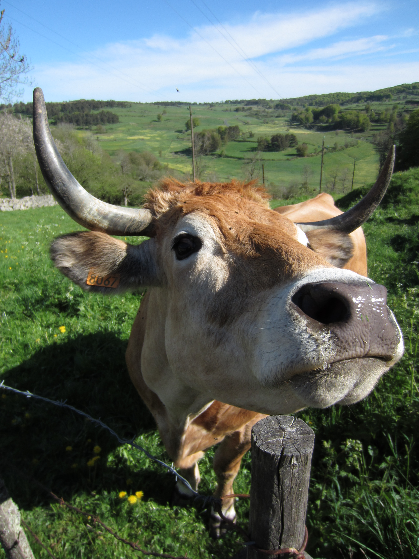
\includegraphics[height=10cm]{figures/speedup}
    \caption{Speedup. Notice that we ran 5 times each simulation and averaged the results.}
    \label{figspeedup}
  \end{center}
\end{figure}

\begin{table}[h!]
  \begin{center}
    %\scriptsize{
    %\scalebox{0.89}{
    \begin{tabular}{>{\columncolor{lightgray}}c|ccc|ccc}
      \hline
      Length of the profiles &  \multicolumn{3}{c}{$20,000$} & \multicolumn{3}{c}{$100,000$} \\
      Number of profiles & 256 & 512 & 1024 & 256 & 512 & 1024\\
      \hline
      Average CPU time (min) & 6 & 15 & 54     & 31 & 70 & 253 \\
      Memory usage (Gb)      & 0.4 & 0.8 & 1.8    &  1.7 & 3.7 & 7.9 \\
      \hline
    \end{tabular}
    %}
    \caption{Average performance of . on $48$ cores (quadri-12 cores Opteron 2.2 GHz + memory
Notice that we ran 5 times each simulation and averaged the results.}
    \label{tabtime}
  \end{center}
\end{table}

\bibliographystyle{plain}
\bibliography{biblio}


\end{document}


\section{Linearized Dynamic Programming to segment individual profiles}
\subsection{Background / Notations}
We consider a signal of length $n$, $\{X_i\}_{i \leq n}$ with $X_i \in \mathbf{R}$.
A segment $r$ is delimited by two change-points and is denoted
 $r = \llbracket t_1, t_2 \rrbracket$.
We define the set of all segmentations of a segment $r$ in $K$ segments as $\mathcal{M}^{(K)}_{(r)} = \mathcal{M}^{(K)}_{t_1, t_2}$.
The $k$-th change of segmentation $m$ in $K$ segments will be denoted by $\tau_k$ with the convention that $\tau_0 = 1$ and $\tau_K = n+1$.
The $k-th$ segment is denoted by $r_k$.
For a given segmentation in $K$ segments we have, $m = \{r_1, r_2 \ldots, r_K\}$ and for all $k \leq K$,  $r_k = \llbracket \tau_k, \tau_{k+1} -1\rrbracket$.

Using the notations of seg-clust (\cite{picard_2007}) the cost of a given segment $r = \llbracket t_1, t_2 \rrbracket$ is given by minus the log-likelihood :
$$ C_{t_1, t_2}^{(1)} =C_{(r)}^{(1)} = -\log\left(\sum_p \pi_p exp\left\{ - \frac{\sum_{i \in r} (x_i - \mu_p)^2 }{ 2 \sigma^2} \right\}\right)$$ 
The optimal cost in $K$ segments from $r = \llbracket t_1, t_2 \rrbracket$ is defined as :
$$C_{t_1, t_2}^{(K)} = C_{(r)}^{(K)} = \min_{m \in \mathcal{M}^{(K)}_{(r)}} \left\{ \sum_{r \in m} C^{(1)}_{(r)} \right\}.$$
The corresponding  optimal segmentation is defined as :
$$\widehat{m}_{t_1, t_2}^{(K)} = \widehat{m}_{(r)}^{(K)} = \underset{m \in \mathcal{M}^{(K)}_{(r)}}{\operatorname{argmin}} \left\{ \sum_{r \in m} C^{(1)}_{(r)} \right\}.$$
The cost or loss of a segmentation is segment additive. Using this segment additivity one can built an $\Theta(Kn^2)$ dynamic programming algorithm to recover the best segmentations (in $1$ to $K$ segments).

Here we propose to approximate this loss in a K-mean fashion
More specifically we propose two possible approximations, the first is:
\begin{eqnarray} \widetilde{C}_{(r)}^{(1)} \approx  \min_p \left\{ \sum_{i \in r}\frac{(x_i - \mu_p)^2} {2\sigma^2 }\right\}
\label{equation:approximation2}\end{eqnarray} 
and the second is 
\begin{eqnarray} \widetilde{C}_{(r)}^{(1)} \approx  \min_p \left\{ \sum_{i \in r}\frac{(x_i - \mu_p)^2} {2\sigma^2 } + \log(\pi_p)\right\} .
\label{equation:approximation1}\end{eqnarray} 
In both cases, $\widetilde{C}_{(r)}^{(K)}$ and $\widetilde{m}_{(r)}^{(K)}$ are defined as:
$$ \widetilde{C}_{(r)}^{(K)} =\min_{m \in \mathcal{M}^{(K)}_{(r)}} \left\{ \sum_{r \in m} \widetilde{C}^{(1)}_{(r)} \right\}, \qquad \text{and} \qquad
 \widetilde{m}_{(r)}^{(K)} = \underset{m \in \mathcal{M}^{(K)}_{(r)}}{\operatorname{argmin}} \left\{ \sum_{r \in m} \widetilde{C}^{(1)}_{(r)} \right\}.$$


%We also have that for all $\tau, \tau' \leq t$ such that
%$$  \widetilde{C}_{(1,\tau)}^{(k)}  +  \widetilde{C}_{(\tau+1, t)}^{(1)}(\mu) \leq  \widetilde{C}_{(1,\tau')}^{(k)}  +  \widetilde{C}_{(\tau'+1, t)}^{(1)}(\mu) $$
% then for any $t' > t$ we have :
%$$  \widetilde{C}_{(1,\tau)}^{(k)}  +  \widetilde{C}_{(\tau+1, t)}^{(1)}(\mu) + \widetilde{C}_{(t+1, t')}^{(1)} \leq  \widetilde{C}_{(1,\tau')}^{(k)}  +  \widetilde{C}_{(\tau'+1, t)}^{(1)}(\mu)  + \widetilde{C}_{(t+1, t')}^{(1)}. $$
%Thus we get that $\forall \tau < t $ : 
%$$  \widetilde{C}_{1, t}^{(k)}(\mu) + \widetilde{C}_{(t+1, t+1)}^{(1)} \leq  \widetilde{C}_{(1,\tau)}^{(k)} + \widetilde{C}_{(\tau+1, t+1)}^{(1)}(\mu).$$
%Thus 
%$$ \min_{\tau < t} \left(  \widetilde{C}_{(1,\tau)}^{k-1}  +  \widetilde{C}_{(\tau+1, t)}^{(1)}(\mu) \right) $$
